\documentclass[12pt, a4paper]{article}
\usepackage{CJKutf8}
\usepackage[left=2cm, right=2cm, top=3cm, bottom=2.5cm]{geometry}
\usepackage[nodayofweek,level]{datetime}
\usepackage{comment}

%..This section controls the header-footer layout of the document
\usepackage{fancyhdr}
\pagestyle{fancy}
\lhead{Machine Learning (NTU CSIE, Fall 2017)}
\chead{}
\rhead{Homework \#1}
\renewcommand{\headrulewidth}{0.4pt}

%..This section controls the title layout
\title{\vspace{-4ex}\bf{\LARGE{Homework \#1}}} 
\author{資工三\space\space\space B04902009\space\space\space 蕭千惠} % \footnote{blablabla} 
\date{\vspace{-2ex}\today\vspace{-4ex}}
%{\formatdate{21}{2}{2017}}

%.. Customize section numbering
% \begin{comment}
\makeatletter
\renewcommand{\@seccntformat}[1]{%
	\ifcsname prefix@#1\endcsname
		\csname prefix@#1\endcsname
	\else
		\csname the#1\endcsname\quad
	\fi
 }
% \newcommand\prefix@section{}{\thesection\space}{Section \thesection: }
% \newcommand\prefix@subsection{}
\makeatother
% \end{comment}
%% \setcounter{secnumdepth}{1} % No numbering
%% \setcounter{secnumdepth}{2} % Start numbering
% \renewcommand\thesubsection{(\arabic{subsection})}

\newcommand\BL[2][$\bullet$]{#1\,\parbox[t]{\levelwidth}{\raggedright#2}}
\def\level#1{\unskip $\left\{\vcenter{\hbox{\shortstack{#1}}}\right.$\ignorespaces}
%.. math
\usepackage{mathtools}
\usepackage{amssymb}
\usepackage{amsmath}

%.. hyperlink / url
\usepackage[hyphens]{url}
\usepackage{hyperref}
\hypersetup{
    colorlinks=true,
    linkcolor=blue,
    filecolor=magenta,      
    urlcolor=blue,
}
\urlstyle{same}
%%\url{url}
%%\herf{url}{words to show}

% .. Include graph
\usepackage{graphicx}
% \includegraphics[width=16.5cm, keepaspectratio=true]{wireless_CSIE_server.png} \par

%.. change font size
\usepackage{type1cm}

%.. change enumerate label
\usepackage{enumitem}
%%\begin{enumerate}[label=(\alph*)]  //(a) (b) (c)
%%\begin{enumerate}[label=(\Alph*)]  //(A) (B) (C)
%%\begin{enumerate}[label=(\roman*)] //(i) (ii) (iii`')
\usepackage{amsfonts}
\usepackage{stmaryrd}

%.. define tab
\newcommand\tab[1][1cm]{\hspace*{#1}}

%.. Content
\begin{document}
	\begin{CJK}{UTF8}{bkai} %use BIG5 enc and bsmi font
	\maketitle\thispagestyle{fancy}
	\linespread{1.5}
	\fontsize{12pt}{10pt} \selectfont

	\section*{Problem 1}
		Score: 200 / 200 \par
		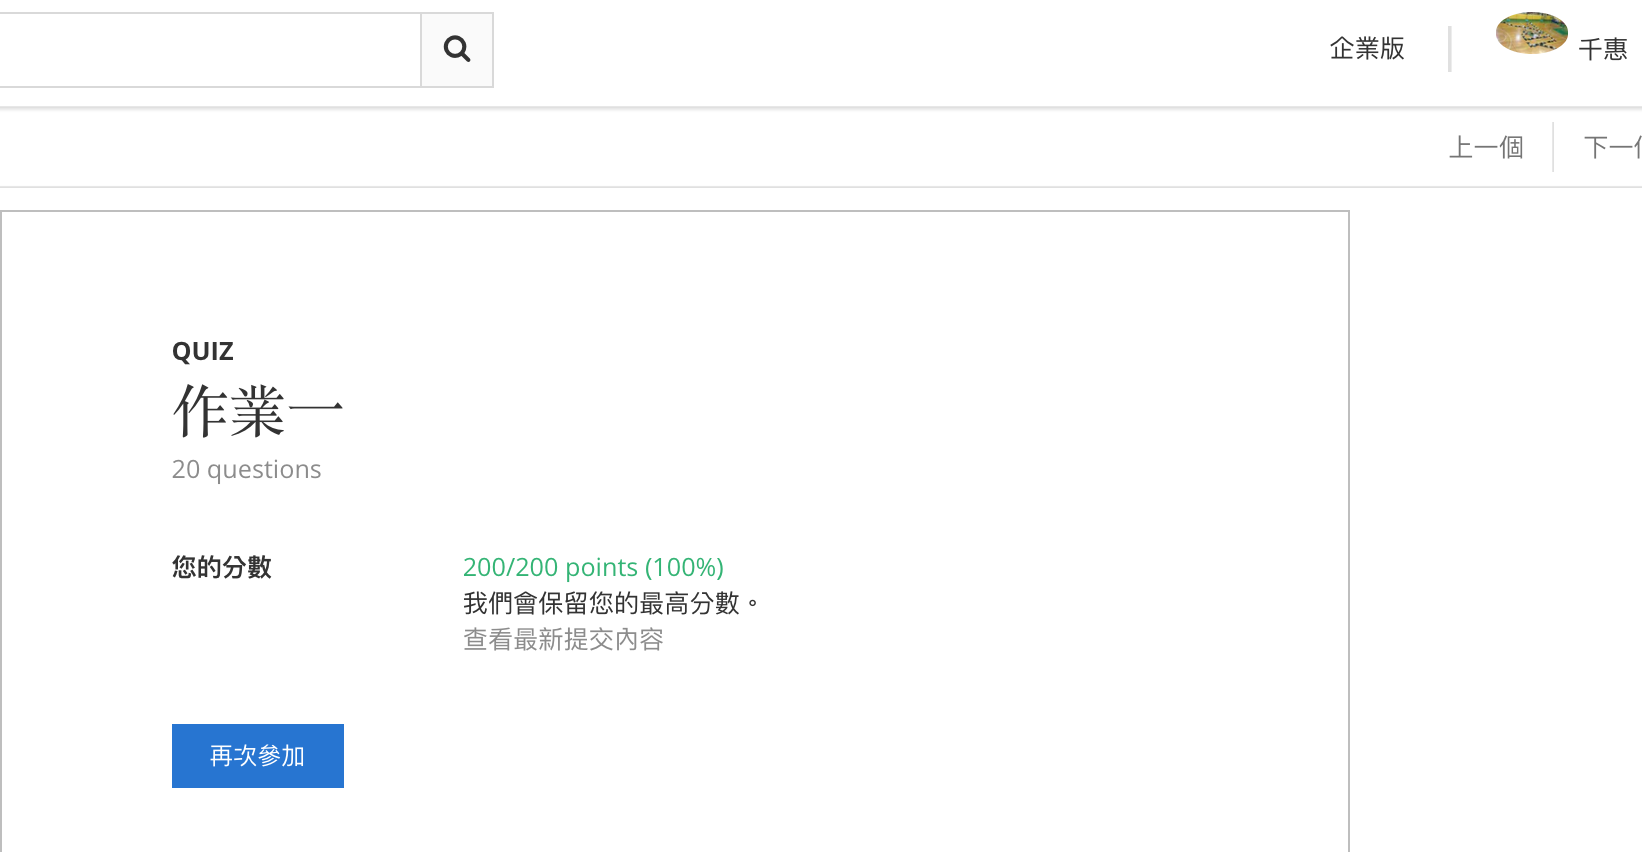
\includegraphics[width=16.5cm, keepaspectratio=true]{1.png} \\
	\section*{Problem 2}
	% Selectively schedule experiments on mice to quickly evaluate the potential of cancer medicines.
	% Cancer study. \par
	\noindent
	Application of active learning: {\bf Redesign of census} \\

	\noindent {\bf Original census}: collects “complete information" from “all participants" in the population. \par
	\hspace{6.5em} All participants are asked to fill out a detailed long form.\\

	\noindent {\bf Census by active learning}:
	\begin{enumerate}
	\item	
		{\bf The algorithm gets a lot of data, but not the labels.} \\
		Ask all participants in the population to fill out a short form. 
		% The short form is created for the algorithm to select  respondents.
	\item
		{\bf Select representative respondents. (A subset of data.)}\\
		The algorithm learns the task and tells what labels would be most useful at the current state.
	\item
		{\bf Manually label just the data in the subset.} \\
	 	Ask the repondents who were selected to fill out a more detailed long form.
	\end{enumerate}
	

	\linespread{1.5}
	\fontsize{12pt}{20pt} \selectfont
	\newpage
	\section*{Problem 3}
		$E_{OTS}(g,f) = \dfrac{1}{L} \sum\limits_{l=1}^{L} \llbracket g(x_{N+l}) \neq f(x_{N+l})\rrbracket$
		$= |\{k \mid N+1\leq k\leq N+L$ and k is even\}$|$ \par
		\begin{enumerate}
			\item
				When N is an even number, let $n_e$ be the number of even number between 1 and L. \\
				$E_{OTS}(g,f) = \dfrac{n_e}{L}$ \\
				$n_e = \lfloor \dfrac{L}{2}\rfloor \\
				 	 = \lfloor \dfrac{L}{2}\rfloor + \lfloor \dfrac{N}{2}\rfloor - \lfloor \dfrac{N}{2}\rfloor \\
					 = \lfloor \dfrac{N+L}{2}\rfloor - \lfloor \dfrac{N}{2}\rfloor$  \hspace{3em}
					(Since $\lfloor \dfrac{N}{2}\rfloor \in \mathbb{N}$, 
				$\lfloor \dfrac{L}{2}\rfloor + \lfloor \dfrac{N}{2}\rfloor = \lfloor \dfrac{N+L}{2}\rfloor$) \\				
				$\Rightarrow E_{OTS}(g,f) = \dfrac{ \lfloor \dfrac{N+L}{2}\rfloor - \lfloor \dfrac{N}{2}\rfloor }{L}$
			\item
				When N is an odd number, let $n_o$ be the number of odd number between 1 and L. \\
				$E_{OTS}(g,f) = \dfrac{n_o}{L}$
				\begin{enumerate}
				\item
					If L is an even number, $n_o = \dfrac{L}{2} \in \mathbb{N}$ \\
					$n_o = \dfrac{L}{2} + \lfloor \dfrac{N}{2}\rfloor - \lfloor \dfrac{N}{2}\rfloor \\
					 = \lfloor \dfrac{N+L}{2}\rfloor - \lfloor \dfrac{N}{2}\rfloor$  \hspace{3em}
					(Since $\dfrac{L}{2} \in \mathbb{N}$)
				\item
					If L is an odd number, $n_o = \dfrac{L+1}{2} \in \mathbb{N}$ \\
					$n_o = \dfrac{L+1}{2} + \lfloor \dfrac{N}{2}\rfloor - \lfloor \dfrac{N}{2}\rfloor \\
					= \dfrac{L+1}{2} + \lfloor \dfrac{N-1}{2}\rfloor - \lfloor \dfrac{N}{2}\rfloor$
					\hspace{3em} (Since N is an odd number, $\lfloor \dfrac{N}{2}\rfloor  = \lfloor \dfrac{N-1}{2}\rfloor $) \\
					$ = \lfloor \dfrac{L+1+N-1}{2}\rfloor - \lfloor \dfrac{N}{2}\rfloor$  \hspace{3.2em}
					(Since $\dfrac{L+1}{2} \in \mathbb{N}$) \\
					$ = \lfloor \dfrac{N+L}{2}\rfloor - \lfloor \dfrac{N}{2}\rfloor$
				\end{enumerate}
				$\Rightarrow E_{OTS}(g,f) = \dfrac{ \lfloor \dfrac{N+L}{2}\rfloor - \lfloor \dfrac{N}{2}\rfloor }{L}$
		\end{enumerate}
		From 1. \& 2., $E_{OTS}(g,f) = \dfrac{ \lfloor \dfrac{N+L}{2}\rfloor - \lfloor \dfrac{N}{2}\rfloor }{L}$

	\newpage
	\section*{Problem 4}
		$f: \mathcal{X}\rightarrow \mathcal{Y}$ , $\mathcal{X} = \{x_1,x_2,x_3,...,x_N,x_{N+1},...x_{N+L}\}$, $\mathcal{Y} = \{-1, +1\}$ \\
		Let $\mathcal{F} = \{f \mid f$ can “generate” $\mathcal{D}$ in a noiseless setting\}  \\
		$\Rightarrow \forall f \in \mathcal{F}$ 
		$\begin{cases}
			(x_i, f(x_i)) \in \mathcal{D} & ,1\leq i\leq N \\
			f(x_i) \in \{-1, +1\}& ,N < i \leq N+L \\
		\end{cases}$ \\
		$\Rightarrow |F| = 1^N * |\{-1,+1\}|^ {(N+L)-N} = 2^L$


	\section*{Problem 5}
		Let $g_1 = \mathcal{A}_1(\mathcal{D})$ and $g_2 = \mathcal{A}_2(\mathcal{D})$ \\
		$E_{OTS}(g,f) = \dfrac{1}{L} \sum\limits_{l=1}^{L} \llbracket g(x_{N+l}) \neq f(x_{N+l})\rrbracket$  \\
		$\mathcal{F}$ is the set of all $f$ that can generate $\mathcal{D}$ in a noiseless setting. $\mathcal{F} = \{f_1,f_2,...f_{2^L}\}$ \\
		$\mathbb{E}_f\Big\{E_{OTS}(g,f)\Big\} = \dfrac{1}{2^L}\sum\limits_{i=1}^{2^L} E_{OTS}(g,f_i)$
		$=\dfrac{1}{2^L}\dfrac{1}{L}\sum\limits_{i=1}^{2^L}\sum\limits_{l=1}^{L} \llbracket g(x_{N+l}) \neq f_i(x_{N+l})\rrbracket$ \\
		$\forall N < k \leq L,$
		$\begin{cases}
			\sum\limits_{i=1}^{2^L}\llbracket f_i(x_k) = 1 \rrbracket = \dfrac{2^{L}}{2} = 2^{L-1}
			\Rightarrow \sum\limits_{i=1}^{2^L}\llbracket f_i(x_k) \neq -1 \rrbracket = 2^{L-1} \\
			\sum\limits_{i=1}^{2^L}\llbracket f_i(x_k) = -1 \rrbracket = \dfrac{2^{L}}{2} = 2^{L-1}
			\Rightarrow \sum\limits_{i=1}^{2^L}\llbracket f_i(x_k) \neq 1 \rrbracket = 2^{L-1} \\
		\end{cases}$ \\
		$\Rightarrow \forall N<k\leq L,\sum\limits_{i=1}^{2^L}\llbracket g(x_k) \neq f_i(x_k)\rrbracket = \sum\limits_{i=1}^{2^L}\Big(\llbracket 1 \neq f(x_k)\rrbracket or \llbracket -1 \neq f(x_k)\rrbracket \Big) = 2^{L-1}$ \\
		$\Rightarrow \mathbb{E}_f\Big\{E_{OTS}(g,f)\Big\} = \dfrac{1}{2^L}\dfrac{1}{L} \sum\limits_{l=1}^{L} 2^{L-1} = \dfrac{1}{2^L}*\dfrac{1}{L}*L*2^{L-1} = \dfrac{1}{2}$ \\
		$\Rightarrow \mathbb{E}_f\Big\{E_{OTS}(\mathcal{A}_1(\mathcal{D}),f)\Big\} = \mathbb{E}_f\Big\{E_{OTS}(\mathcal{A}_2(\mathcal{D}),f)\Big\} = \dfrac{1}{2}$ 

	\section*{Problem 6}
		If B or D dice is picked, we get green 1’s. Otherwise, we get orange 1's. \\
		$\Rightarrow$ For every pick, the probability of getting a green 1's is $\dfrac{2}{4} = \dfrac{1}{2}$\\
		$\Rightarrow$ Picking five dices, the probability of getting five green 1's is $(\dfrac{1}{2})^5 = \dfrac{1}{32}$
	
	\section*{Problem 7}
		The target is to get “some number” that is purely green when picking 5 dice from the bag. \\ $\Rightarrow$ Dice A and dice B can't be picked together. \par
		Dice C and dice D can't be picked together either.
		\begin{enumerate}
		\item
			Picking only one kind of dices. $\Rightarrow P = 4 * (\dfrac{1}{4})^5 = \dfrac{1}{256}$
		\item
			Picking two kinds of dices: (A\&C) or (A\&D) or (B\&C) or (B\&D) \\
			$\Rightarrow P = 4*[(\dfrac{2}{4})^5 - 2 * (\dfrac{1}{4})^5] = \dfrac{30}{256} $
		\end{enumerate}
		$\Rightarrow$ When picking 5 dice from the bag, the total probability of getting “some number” that is purely green is $\dfrac{1}{256}+\dfrac{30}{256}=\dfrac{31}{256}$

	\section*{Problem 8}
		Average number of updates: 39 \\
		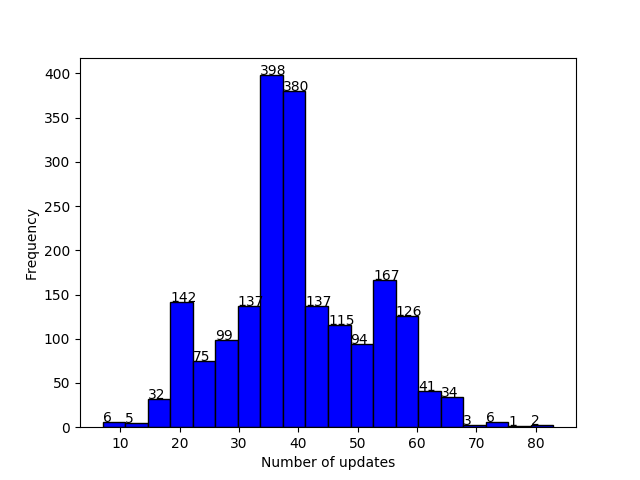
\includegraphics[width=14cm, keepaspectratio=true]{8.png} \par
	
	\section*{Problem 9(Bonus)}
		$R^2 = \max\limits_{n} ||{\bf x}_n||^2$, 
		$\rho = \min\limits_{n}y_n  \dfrac{{\bf w}_{f}^{T}}{||{\bf w}_f||}{\bf x}_n$, 
		$T \leq \dfrac{R^2}{\rho^2}$ \\
		When scaling down all ${\bf x}_n$ linearly by a factor of 20, \\
		$\begin{cases}
			\max\limits_{n}||{\bf x'}_n|| = \dfrac{1}{20}\max\limits_{n}||{\bf x}_n ||
			\rightarrow (R')^2 = (\dfrac{1}{20})^2 R^2 \\
			\min\limits_{n}||{\bf x'}_n|| = \dfrac{1}{20}\min\limits_{n}||{\bf x}_n ||
			\rightarrow \rho' =  \dfrac{1}{20} \rho\\
		\end{cases}$ \\
		$\Rightarrow T' \leq \dfrac{(R')^2}{(\rho')^2} = \dfrac{(\dfrac{1}{20}R)^2}{(\dfrac{1}{20}\rho)^2} = \dfrac{R^2}{\rho^2}$ \\
		$\Rightarrow$ PLA algorithm would not run 20 times faster.


	\clearpage
	\end{CJK}
\end{document}